\subsection{StrongSORT}

StrongSORT -- алгоритм трекинга, являющийся улучшением алгоритма DeepSORT, который, получая на вход данные с этапа детектирования, использует дескриптор описания объектов для получения особенностей изображений объектов и  построения коэффициента сходства между траекторией и новым срабатыванием детектора, повышая качество отслеживания объектов.

\vspace{0.3cm}

\begin{figure}[ht]
    \centering
    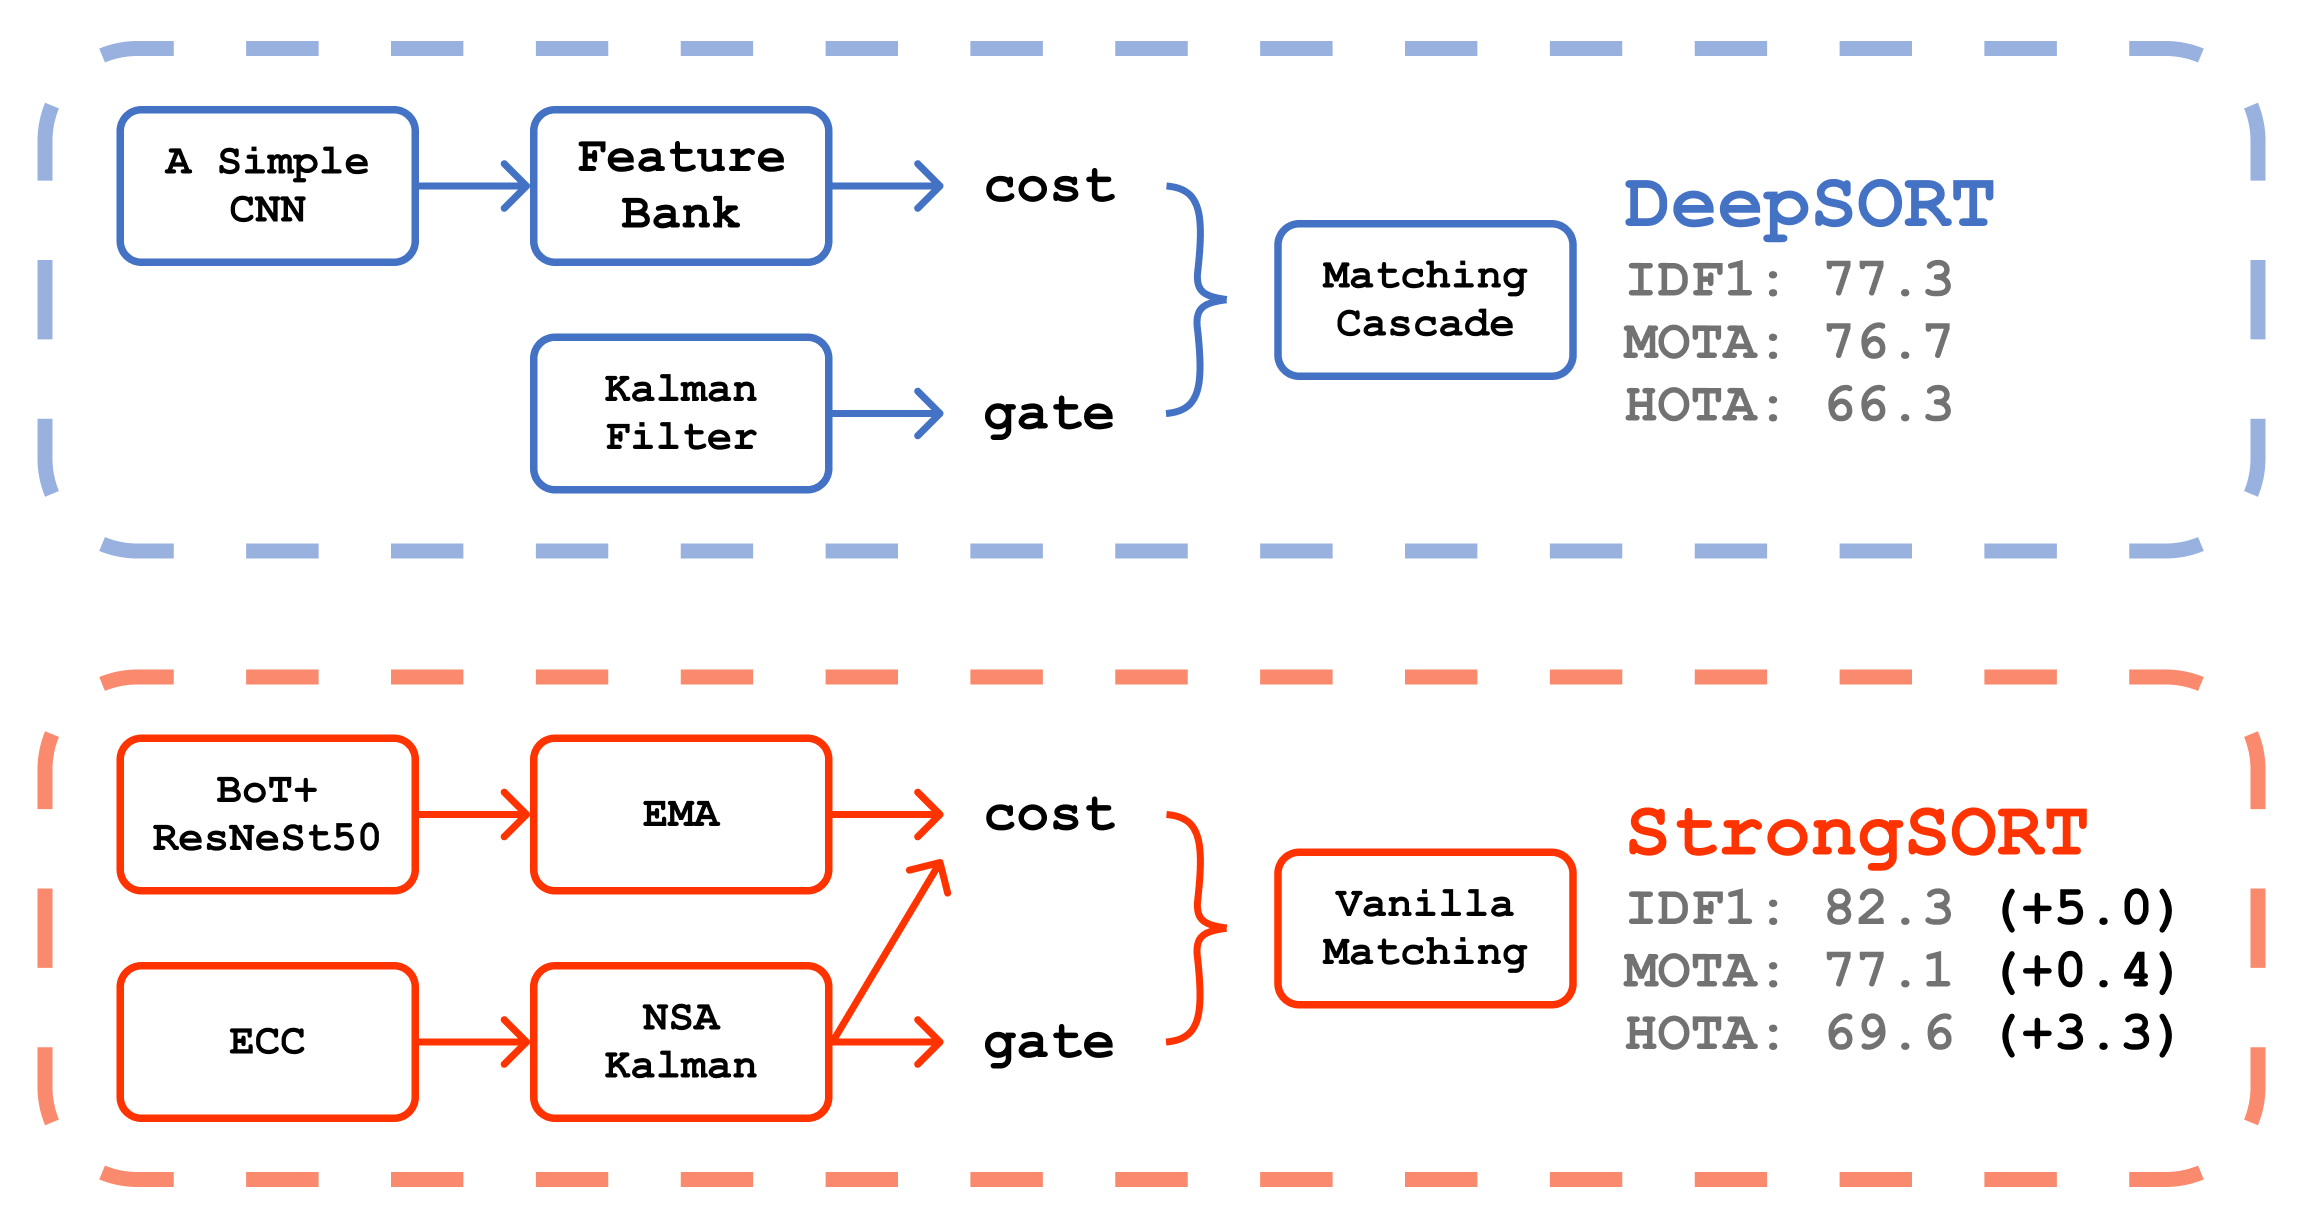
\includegraphics[width=0.85\textwidth]{7-1}
    \caption{Сравнение DeepSORT и StrongSORT}
    \label{img:7-1}
\end{figure}

\textbf{Улучшенные модули.} Faster R-CNN и CNN из DeepSORT заменены на YOLOX-X \cite{7-1} и BoT \cite{7-2}, позволяющие извлекать большее количество признаков объектов.

\vspace{0.2cm}

\textbf{EMA (Exponential Moving Average).} Механизм feature bank, чувствительный к шуму \cite{7-3}, заменяется новой стратегией обновления признаков, использующей межкадровую информацию и снижающей уровень шума при обнаружении, что не только улучшает качество сопоставления, но и сокращает временные затраты \cite{7-4}.

\vspace{0.2cm}

\textbf{ECC (Enhanced Correlation Coefficient).} Для уменьшения влияния движения камеры вводится метод параметрического выравнивания изображений, оценивающий глобальное изменение движения камеры между кадрами \cite{7-5}. Его основу представляет следующий критерий для количественной оценки работы межкадрового преобразования:

    \begin{equation}
        E_{ECC}(p) = \norm{ \frac{\bar{i}_r}{\norm{\bar{i}_r}} - \frac{\bar{i}_w(p)}{\norm{\bar{i}_w(p)}} }^2,
    \end{equation}

\noindent где $\norm{\cdot}$ -- евклидова норма, $p$ -- параметр преобразования, $\bar{i}_r$ и $\bar{i}_w(p)$ -- изначальное и преобразованное изображения с нулевым средним. Далее задача выравнивания решается путем минимизации $E_{ECC}(p)$ с предложенным прямым аддитивным итерационным алгоритмом или обратным композиционным итерационным алгоритмом.

\vspace{0.2cm}

\textbf{NSA Kalman.} Классическая версия фильтра Калмана чувствительна к обнаружениям плохого качества и игнорирует информацию о масштабах шума обнаружения \cite{7-6}. Решением этой проблемы служит NSA Калман из GIAOTracker, предлагающий формулу для адаптивного вычисления шума ковариации $\bar{R_k}=(1-c_k)R_k$, где $R_k$ -- константа шума ковариации по умолчанию, а $c_k$ -- оценка достоверности на шаге $k$. Очевидно, что более высокая оценка $c_k$ соответствует более низкому уровню шума, что и сказывается на низком $\bar{R_k}$.

\vspace{0.2cm}

\textbf{Motion Cost.} Используется как информация о внешнем облике объекта, так и информация о его передвижении.

\vspace{0.2cm}

\textbf{Vanilla Matching.} Каскадный алгоритм \cite{7-7} ограничивает производительность трекера, делая его чувствительным к запутанным ассоциациям. В качестве решения данной проблемы он заменяется на алгоритм Vanilla Global Linear Assignment.

\vspace{0.2cm}

\textbf{AFLink.} Для достижения ассоциаций высокой точности во множестве работ часто используется глобальная связь для треклетов. Однако они требуют больших вычислительных затрат и имеют множество гиперпараметров для точной настройки. Например, алгоритм связей в GIAOTracker использует улучшенный ResNet50-TP для извлечения 3D признаков треклетов и выполнения ассоциации с дополнительными пространственными и временными расстояниями. Ему необходимо установить 6 гиперпараметров, что влечет за собой продолжительные эксперименты по настройке и низкую устойчивость. Исходя из этого, предлагается модель, не использующая информацию о внешнем виде, предсказывающая связь объектов между треклетами, полагаясь только на пространственно-временную информацию.
